% !TEX TS-program = pdflatex
% !TEX encoding = UTF-8 Unicode

% This is a simple template for a LaTeX document using the "article" class.
% See "book", "report", "letter" for other types of document.

\documentclass[11pt]{article} % use larger type; default would be 10pt

\usepackage[utf8]{inputenc} % set input encoding (not needed with XeLaTeX)

%%% Examples of Article customizations
% These packages are optional, depending whether you want the features they provide.
% See the LaTeX Companion or other references for full information.

%%% PAGE DIMENSIONS
\usepackage{geometry} % to change the page dimensions
\geometry{a4paper} % or letterpaper (US) or a5paper or....
% \geometry{margin=2in} % for example, change the margins to 2 inches all round
% \geometry{landscape} % set up the page for landscape
%   read geometry.pdf for detailed page layout information

\usepackage{graphicx} % support the \includegraphics command and options
\graphicspath{ {./Figs/} }  % requires additional {} and trailing '/'!


% \usepackage[parfill]{parskip} % Activate to begin paragraphs with an empty line rather than an indent

%%% PACKAGES
\usepackage{booktabs} % for much better looking tables
\usepackage{array} % for better arrays (eg matrices) in maths
\usepackage{paralist} % very flexible & customisable lists (eg. enumerate/itemize, etc.)
\usepackage{verbatim} % adds environment for commenting out blocks of text & for better verbatim
\usepackage{subfig} % make it possible to include more than one captioned figure/table in a single float

\usepackage{colortbl}

\usepackage{amsmath}
\usepackage{xifthen}
\usepackage{tikz}
\usepackage{relsize}
\usetikzlibrary{matrix}
\usetikzlibrary{positioning}
\usetikzlibrary{calc}
\usetikzlibrary{shapes}

\usepackage{theorem}
\newtheorem{definition}{Definition}


% These packages are all incorporated in the memoir class to one degree or another...

%%% HEADERS & FOOTERS
\usepackage{fancyhdr} % This should be set AFTER setting up the page geometry
\pagestyle{fancy} % options: empty , plain , fancy
\renewcommand{\headrulewidth}{0pt} % customise the layout...
\lhead{}\chead{}\rhead{}
\lfoot{}\cfoot{\thepage}\rfoot{}

%%% SECTION TITLE APPEARANCE
\usepackage{sectsty}
\allsectionsfont{\sffamily\mdseries\upshape} % (See the fntguide.pdf for font help)
% (This matches ConTeXt defaults)

%%% ToC (table of contents) APPEARANCE
\usepackage[nottoc,notlof,notlot]{tocbibind} % Put the bibliography in the ToC
\usepackage[titles,subfigure]{tocloft} % Alter the style of the Table of Contents
\renewcommand{\cftsecfont}{\rmfamily\mdseries\upshape}
\renewcommand{\cftsecpagefont}{\rmfamily\mdseries\upshape} % No bold!

%%% END Article customizations

\newcommand{\ub}{\text{{\tt.}}}

\tikzstyle{bp}=[line width=5pt,draw=blue, opacity=.6,in =90,out=90,looseness=1.5]
\tikzstyle{altbp}=[line width=5pt,draw=red, opacity=.6, in =-90,out=-90,looseness=1.5]
\tikzstyle{cell}=[inner sep=2]
\tikzstyle{backbone}=[line width=2pt]
\tikzstyle{every picture}+=[remember picture]

\def\mySecStr#1{\expandafter {\tt #1}\& }
\def\mySecStrAll#1{\ifx#1\mySecStrAll\else\mySecStr#1\expandafter\mySecStrAll\fi}
\def\mySeq#1{\expandafter {\relsize{-2}\sf #1}\&}
\def\mySeqAll#1{\ifx#1\mySeqAll\else\mySeq#1\expandafter\mySeqAll\fi}


\newcommand{\RNA}[3][]{
\begin{tikzpicture}[baseline={([yshift=-.5ex]rna)}]
  \matrix[matrix of nodes,nodes=cell,ampersand replacement=\&] (rna){
		\mySecStrAll #2 \mySecStrAll\\
		};
\ifthenelse{\equal{#3}{}}{}{%
	\foreach \x/\y in {#3}{\draw (rna-1-\x) edge[bp] (rna-1-\y);}%
}
\ifthenelse{\equal{#1}{}}{}{%
		\foreach \x/\y in {#1}{\draw (rna-1-\x) edge[altbp] (rna-1-\y);}%
		}
\end{tikzpicture}} 

\setlength{\parskip}{1em}
\renewcommand{\H}[1]{{\tt#1}}

\newcommand{\Summary}{
  \tikzstyle{bp}=[line width=5pt,draw=red!50!blue, opacity=.6,in =90,out=90,looseness=1.5]
  \tikzstyle{altbp}=[line width=5pt,draw=red!50!blue, opacity=.6, in =90,out=90,looseness=1.5]
}


\newcommand{\Case}[3]{\item $\{#1\}$: {\sf #3}-type

{\centering 
#2 $\longrightarrow$\Summary#2\\}

}

\newcommand{\SW}[1]{\textbf{SW-}#1}

%% graphical notation of grammar rules with tikz
\newcommand{\GRgaplength}{0.9}
\newcommand{\GRsubseqlength}{0.35}
\newcommand{\GRarcratio}{0.8}
\newcommand{\GRdecwfraglength}{0.4}
\newcommand{\GRunitlength}{0.15} % distance between concatenated fragments

\usetikzlibrary{decorations.pathmorphing}

\tikzstyle{very densely dashed} = [dash pattern=on 2.5pt off 1.5pt]
%\tikzstyle{very densely dashed} = [thin,decorate, decoration={snake,segment length=1.5mm, amplitude=0.3mm}]%[dash pattern=on 2.5pt off 1.5pt]

%% --------------------------------------------------------------------------- 
%% Gapped fragments

% draw base of gapped fragment (without arcs)
\newcommand{\GRgapfragBase}[2][]{%
  \path[draw=none]
    (last)                node (i) [scale=0.1] {}
    ++(\GRsubseqlength,0) node (j) [scale=0.1] {}
    ++(\GRgaplength,0)    node (k) [scale=0.1] {}
    ++(\GRsubseqlength,0) node (l) [scale=0.1] {};
%
  \draw [backbone]
      (i) -- (j)
      (k) -- (l);
%
  \draw (j) edge [draw=none] node [below] (label) {#2} (k); 
%
  \node (last) at (l) {};
}

%draw the points at i,j,k,l for the gapped fragment
\newcommand{\GRgapfragPoints}[1][]{%
  \path[itype/.style=fix,
        jtype/.style=fix,
        ktype/.style=fix,
        ltype/.style=fix,
        #1]
    (i) node [itype] () {}
    (j) node [jtype] () {}
    (k) node [ktype] () {}
    (l) node [ltype] () {};
}

%draw arcs of gapped fragment
\newcommand{\GRgapfragOuterArc}[1]{%
  \pgfmathsetmacro\outerradiusX{(\GRgaplength+2*\GRsubseqlength)/2}
  \pgfmathsetmacro\outerradiusY{\outerradiusX*\GRarcratio}

  \draw[arc,#1]
    (i) arc [radius=\outerradiusX, y radius=\outerradiusY, start angle=180,end angle=0];
}

\newcommand{\GRgapfragInnerArc}[1]{
  \pgfmathsetmacro\innerradiusX{\GRgaplength/2}
  \pgfmathsetmacro\innerradiusY{\innerradiusX*\GRarcratio}
  \draw[arc,#1]
    (j) arc [x radius=\innerradiusX, y radius=\innerradiusY, start angle=180,end angle=0];
}

% draw dashed inner and outer arcs
\newcommand{\GRgapfragArcs}{%
  \GRgapfragInnerArc{very densely dashed}
  \GRgapfragOuterArc{very densely dashed}
}

%% draw a gapped fragment
\newcommand{\GRgapfrag}[2][]{%
  \GRgapfragBase[#1]{#2}
  \GRgapfragArcs
  \GRgapfragPoints[#1]
}

\newcommand{\GRgapfragArcsL}{%
  \GRgapfragArcs
  \draw (i) edge [in=90,out=90,arc] (j);
}
\newcommand{\GRgapfragArcsM}{%
  \GRgapfragInnerArc{solid}
  \GRgapfragOuterArc{very densely dashed}
}
\newcommand{\GRgapfragArcsR}{%
  \GRgapfragArcs
  \draw (k) edge [in=90,out=90,arc] (l);
}
\newcommand{\GRgapfragArcsO}{%
  \GRgapfragInnerArc{very densely dashed}
  \GRgapfragOuterArc{solid}
}

\newcommand{\GRgapfragArcsfromL}{%
  \GRgapfragArcs
  \draw (i) edge [in=90,out=90,arc,dotted] (j);
}
\newcommand{\GRgapfragArcsfromM}{%
  \GRgapfragInnerArc{dotted}
  \GRgapfragOuterArc{very densely dashed}
}
\newcommand{\GRgapfragArcsfromR}{%
  \GRgapfragArcs
  \draw (k) edge [in=90,out=90,arc,dotted] (l);
}
\newcommand{\GRgapfragArcsfromO}{%
  \GRgapfragInnerArc{very densely dashed}
  \GRgapfragOuterArc{dotted}
}

\newcommand{\GRsingleOfrag}{%
  \path[draw=none]
    (last)                node (i) [scale=0.1] {}
    ++(\GRsubseqlength,0) node (j) [scale=0.1] {}
    ++(\GRgaplength,0)    node (k) [scale=0.1] {}
    ++(\GRsubseqlength,0) node (l) [scale=0.1] {};

  \GRgapfragOuterArc{solid}

  \path[itype/.style=fix,
        ltype/.style=fix]
    (i) node [itype] () {}
    (l) node [ltype] () {};
}

\newcommand{\GRgapfragDecorate}{%
}

\newcommand{\GRgapfragDecoratelO}{%
  \pgfmathsetmacro\radiusX{(\GRgaplength+1.5*\GRsubseqlength)/2}
  \pgfmathsetmacro\radiusY{\radiusX*\GRarcratio}
  \draw (i) [arc] arc [x radius=\radiusX, y radius=\radiusY, start angle=180,end angle=0];
}

\newcommand{\GRgapfragDecorateLo}{%
  \pgfmathsetmacro\radiusX{(0.6*\GRsubseqlength)/2}
  \pgfmathsetmacro\radiusY{\radiusX*\GRarcratio}
  \draw (i) [arc] arc [x radius=\radiusX, y radius=\radiusY, start angle=180,end angle=0];
}

\newcommand{\GRgapfragDecoraterO}{%
  \pgfmathsetmacro\radiusX{(\GRgaplength+1.5*\GRsubseqlength)/2}
  \pgfmathsetmacro\radiusY{\radiusX*\GRarcratio}
  \draw (l) [arc] arc [x radius=\radiusX, y radius=\radiusY, start angle=0,end angle=180];
}

\newcommand{\GRgapfragDecorateRo}{%
  \pgfmathsetmacro\radiusX{(0.6*\GRsubseqlength)/2}
  \pgfmathsetmacro\radiusY{\radiusX*\GRarcratio}
  \draw (l) [arc] arc [x radius=\radiusX, y radius=\radiusY, start angle=0,end angle=180];
}

\newcommand{\GRgapfragDeco}[4][]{%
  \GRgapfragBase{#2}
  \csname GRgapfragArcs#3\endcsname
  \csname GRgapfragDecorate#4\endcsname
  \GRgapfragPoints[#1]
}

\newcommand{\GRdecwfrag}[2][]{%
  \path%
    (last) node [scale=0.1]    (i) {}%
    ++(\GRdecwfraglength,0) node [scale=0.1] (l) {};%
  % 
  \draw[very densely dashed,thick] (i) arc (180:0:0.2);%
  %
  \draw [backbone,
        itype/.style={draw=none},
        ltype/.style={draw=none},
        label/.style={below},
        #1]
        (i) node [itype] () {} 
        -- node [label] (label){#2} ++ (0.4,0) 
        node [ltype] () {};%
  \node (last) at (l) {};%
}

\newcommand{\GRsetlast}[2][0]{%
  \path (last) node (bkplast) {}%
    (#2) ++(#1,0) node (last) {};%
}
\newcommand{\GRrestorelast}{%
  \path (bkplast) node (last) {};%
}
\newcommand{\GRconcat}{%
  \path (last) ++(\GRunitlength,0) node (last) {};
}
\newcommand{\GRconcatWAfter}[1]{%
  \GRsetlast[\GRunitlength]{#1}%
}
\newcommand{\GRconcatWBefore}[1]{%
  \pgfmathsetmacro\offset{\GRdecwfraglength+\GRunitlength}
  \GRsetlast[-\offset]{#1}%
}

\newcommand{\GRnewrule}{%
  \path (start) ++(0,-1.5) node (last) {}%
        (last) node (start) {};%
}

% secondary label
\newcommand{\GRseclabel}[1]{%
  \path (l) + (-0.3,0.6) node [text ragged,anchor=west,align=left] (label) {#1};%
  \path (label.east) ++ (-0.2,-0.6) node (last) [] {};%
}

\newcommand{\GRdecompTo}{%
  \draw (last) ++(0.2,0.3) edge [->,very thick] ++(0.9,0);
  \path (last) ++(1.4,0) node (last) {};
}

\newcommand{\GRor}{%
  \draw (last) ++(0.3,0) edge [very thick] ++(0,0.8);
  \path (last) ++(0.6,0) node (last) {};
}

%% Decompositions into W-like fragment and gapped fragment
% decomposition, split at i
\newcommand{\GRgapfragWDecompI}[5][]{%
  \GRdecwfrag[itype/.style=fix,label/.style={above=0.15},#1]{#5}\GRconcat
  \GRgapfragDeco[itype/.style=free,#1]{#2}{#3}{#4}
}
\newcommand{\GRgapfragWDecompJ}[5][]{%
  \GRgapfragDeco[jtype/.style=free,#1]{}{#3}{#4}
  \GRseclabel{#2}
  \GRconcatWAfter{j}\GRdecwfrag[ltype/.style=fix,#1]{#5}\GRrestorelast
}
\newcommand{\GRgapfragWDecompK}[5][]{%
  \GRgapfragDeco[ktype/.style=free,#1]{}{#3}{#4}
  \GRseclabel{#2}
  \GRconcatWBefore{k}\GRdecwfrag[itype/.style=fix,#1]{#5}\GRrestorelast
}
\newcommand{\GRgapfragWDecompL}[5][]{%
  \GRgapfragDeco[ltype/.style=free,#1]{#2}{#3}{#4}
  \GRconcat\GRdecwfrag[ltype/.style=fix,label/.style={above=0.15},#1]{#5}
}

\newenvironment{GRule}{%
  \begin{tikzpicture}[fix/.style={fill,circle,scale=0.4,red!50!black!90},
                      free/.style={fill,rectangle,scale=0.55,blue!60!black!80},
                      backbone/.style={very thick},
                      arc/.style={thick}]
  \node (start) at (0,0) {};
  \node (last) at (0,0) {};
}{%
  \end{tikzpicture}%
}



%%% The "real" document content comes below...

\title{A sketch of unambiguous DP for CCJ}
\author{Hosna, Sebastian, Yann}
%\date{} % Activate to display a given date or no date (if empty),
         % otherwise the current date is printed 



\begin{document}
\maketitle


% The original DP decomposition underlying the CCJ algorithm is ambiguous on multiple levels.
% {\em Can we lift this ambiguity without too much hassle?}
% A key element in the decomposition, and one of the major source of ambiguity, resides in the assembly of two \emph{gapped} pseudoknotted elements, akin to the 3-band/kissing hairpin motif. However, in order to achieve maximum expressivity, only the middle helix is mandatory within each gapped element, meaning that some structure may be obtained in several different ways. In this short note, we explore the different combinations, and build a minimal subset of structures, built from combinations of atomic gapped structures that captures the same search space within inducing any ambiguity.

% Let us first introduce a bit of nomenclature. The helices in the first gapped structure are named \H{1}, \H{2} and \H{3} (resp. \H{A}, \H{B} and \H{C}), as illustrated below:

% {\centering 
% \RNA[4/6,5/11,10/12]{121ABA323CBC}{1/3,2/8,7/9}\\}

% \noindent Note that each helix must contain at least one base pair and, in the case where it contains internal loops and recursive subtructures\footnote{Are those allowed anyway?} must start and finish with a base pair (potentially the same if restricted to a single base pair).

% In order to avoid ambiguity at a higher level in the decomposition, it is crucial that the base pairs in the assembly of gapped elements form a unique connected component in the conflict graph induced by the crossing relationship. Indeed, disconnected components correspond to part in a pseudoknot that can be generated either by sequential composition, or by a recursive call, generating a nested subcomponent. It is thus easy to say that helices \H{2} and \H{B} cannot be omitted. Conversely, helices \H{1}, \H{3}, \H{A}, and \H{C} represent leaves of the conflict graph, and can therefore be safely discarded without disconnecting the conflict graph, \emph{i.e.} without inducing any ambiguity.

% We are left to systematically explore the subsets of $\{\H{1}, \H{3}, \H{A}, \H{C}\}$, in combination with the two mandatory helices \H{2} and \H{B}:
% \begin{itemize} 
% \item Second component is $\{\H{B}\}$:
% \begin{itemize} 
% \Case{\H{2}, \H{B}}{\RNA[5/11]{-2--B--2--B-}{2/8}}{H}
% \Case{\H{1},\H{2}, \H{B}}{\RNA[5/11]{121-B--2--B-}{1/3,2/8}}{KH}
% \Case{\H{2}, \H{3}, \H{B}}{\RNA[5/11]{-2--B-323-B-}{2/8,7/9}}{H}
% {\bfseries Note:} Second band features at least 2 base pairs
% \Case{\H{1},\H{2}, \H{3}, \H{B}}{\RNA[5/11]{121-B-323-B-}{1/3,2/8,7/9}}{KH}
% {\bfseries Note:} Third band features at least 2 base pairs
% \end{itemize} 
% \item Second component is $\{\H{A},\H{B}\}$:
% \begin{itemize} 
% \Case{\H{2}, \H{A}, \H{B}}{\RNA[4/6,5/11]{-2-ABA-2--B-}{2/8}}{H}
% {\bfseries Note:} First band features at least 2 base pairs
% \Case{\H{1},\H{2}, \H{A}, \H{B}}{\RNA[4/6,5/11]{121ABA-2--B-}{1/3,2/8}}{KH$^{\text{a}}$}
% \Case{\H{2}, \H{3}, \H{A}, \H{B}}{\RNA[4/6,5/11]{-2-ABA323-B-}{2/8,7/9}}{H$^{\text{a}}$}
% \Case{\H{1},\H{2}, \H{3}, \H{A}, \H{B}}{\RNA[4/6,5/11]{121ABA323-B-}{1/3,2/8,7/9}}{KH$^{\text{b}}$}
% \end{itemize} 
% \item Second component is $\{\H{B},\H{C}\}$:
% \begin{itemize} 
% \Case{\H{2}, \H{B}, \H{C}}{\RNA[5/11,10/12]{-2--B--2-CBC}{2/8}}{KH}
% \Case{\H{1},\H{2}, \H{B}, \H{C}}{\RNA[5/11,10/12]{121-B--2-CBC}{1/3,2/8}}{4B}
% \Case{\H{2}, \H{3}, \H{B}, \H{C}}{\RNA[5/11,10/12]{-2--B-323CBC}{2/8,7/9}}{KH$^{\text{c}}$}
% \Case{\H{1},\H{2}, \H{3}, \H{B}, \H{C}}{\RNA[5/11,10/12]{121-B-323CBC}{1/3,2/8,7/9}}{4B$^{\text{a}}$}
% \end{itemize} 
% \item Second component is $\{\H{A},\H{B},\H{C}\}$:
% \begin{itemize} 
% \Case{\H{2}, \H{A}, \H{B}, \H{C}}{\RNA[4/6,5/11,10/12]{-2-ABA-2-CBC}{2/8}}{KH}
% {\bfseries Note:} First band features at least 2 base pairs
% \Case{\H{1},\H{2}, \H{A}, \H{B}, \H{C}}{\RNA[4/6,5/11,10/12]{121ABA-2-CBC}{1/3,2/8}}{4B$^{\text{b}}$}
% \Case{\H{2}, \H{3}, \H{A}, \H{B}, \H{C}}{\RNA[4/6,5/11,10/12]{-2-ABA323CBC}{2/8,7/9}}{KH$^{\text{d}}$}
% \Case{\H{1},\H{2}, \H{3}, \H{A}, \H{B}, \H{C}}{\RNA[4/6,5/11,10/12]{121ABA323CBC}{1/3,2/8,7/9}}{CCJ}
% \end{itemize}
% \end{itemize}

% \begin{table}
% { 
%   \tikzstyle{cell}=[inner sep=1.2]
%   \tikzstyle{bp}=[line width=2pt,draw=red!50!blue!80!white, opacity=1,in =90,out=90,looseness=1.3]
%   \tikzstyle{altbp}=[line width=2pt,draw=red!50!blue!80!white, opacity=1, in =90,out=90,looseness=1.3]
% \centering\begin{tabular}{@{}ll@{}ll@{}l@{}}\toprule
% Type & Helix classes && Subsets (sort of)&\\ \midrule
% {\sf H} & $\{\H{2},\H{B}\}$ &\RNA[5/11]{-2--B--2--B-}{2/8}& $\{\H{2},\H{3},\H{B}\}$&\RNA[5/11]{-2--B-323-B-}{2/8,7/9}\\ 
% & &  & $\{\H{2},\H{A},\H{B}\}$  &\RNA[4/6,5/11]{-2-ABA-2--B-}{2/8}\\ 
% \arrayrulecolor{gray!60}\midrule
% {\sf H}$^{\text{a}}$ & $\{\H{2}, \H{3}, \H{A}, \H{B}\}$&\RNA[4/6,5/11]{-2-ABA323-B-}{2/8,7/9} &  &\\ 
% \arrayrulecolor{black}\midrule
% {\sf KH} & $\{\H{1},\H{2},\H{B}\}$&\RNA[5/11]{121-B--2--B-}{1/3,2/8} & $\{\H{1},\H{2},\H{3},\H{B}\}$  &\RNA[5/11]{121-B-323-B-}{1/3,2/8,7/9}\\ 
%  & $\{\H{2},\H{B},\H{C}\}$ &\RNA[5/11,10/12]{-2--B--2-CBC}{2/8} & $\{\H{2},\H{A},\H{B},\H{C}\}$  &\RNA[4/6,5/11,10/12]{-2-ABA-2-CBC}{2/8}\\ 
% \arrayrulecolor{gray!60}\midrule
% {\sf KH}$^{\text{a}}$ & $\{\H{1},\H{2}, \H{A}, \H{B}\}$&\RNA[4/6,5/11]{121ABA-2--B-}{1/3,2/8} &  & \\ 
% {\sf KH}$^{\text{b}}$ & $\{\H{1},\H{2}, \H{3}, \H{A}, \H{B}\}$&\RNA[4/6,5/11]{121ABA323-B-}{1/3,2/8,7/9} &  &\\ 
% {\sf KH}$^{\text{c}}$ & $\{\H{2}, \H{3}, \H{B}, \H{C}\}$&\RNA[5/11,10/12]{-2--B-323CBC}{2/8,7/9} &  & \\ 
% {\sf KH}$^{\text{d}}$ & $\{\H{2}, \H{3}, \H{A}, \H{B}, \H{C}\}$&\RNA[4/6,5/11,10/12]{-2-ABA323CBC}{2/8,7/9} &  & \\ 
% \arrayrulecolor{black}\midrule
% {\sf 4B} & $\{\H{1},\H{2},\H{B},\H{C}\}$&\RNA[5/11,10/12]{121-B--2-CBC}{1/3,2/8}  &  &\\ 
% \arrayrulecolor{gray!60}\midrule
% {\sf 4B}$^{\text{a}}$ & $\{\H{1},\H{2}, \H{3}, \H{B}, \H{C}\}$&\RNA[5/11,10/12]{121-B-323CBC}{1/3,2/8,7/9} &  & \\ 
% {\sf 4B}$^{\text{b}}$ & $\{\H{1},\H{2}, \H{A}, \H{B}, \H{C}\}$&\RNA[4/6,5/11,10/12]{121ABA-2-CBC}{1/3,2/8} &  & \\ 
% \arrayrulecolor{black}\midrule
% {\sf CCJ} & $\{\H{1},\H{2},\H{3},\H{A},\H{B},\H{C}\}$&\RNA[4/6,5/11,10/12]{121ABA323CBC}{1/3,2/8,7/9} &  &\\ 
% \bottomrule
% \end{tabular}\\}

% \caption{Isomorphism classes for relevant subsets of {\sf CCJ} helices}\label{tab:iso}
% \end{table}

% We summarize in Table~\ref{tab:iso} the various accessible classes. A close inspection of the classes reveals two -- complete and unambiguous -- decompositions of the CCJ class in the following subsets of non-empty helices:

% {\centering$\{\H{2},\H{B}\}$, 
% $\{\H{2}, \H{3}, \H{A}, \H{B}\}$, 
% $\{\H{1},\H{2},\H{B}\}$ \emph{or} $\{\H{2},\H{B},\H{C}\}$,
% $\{\H{1},\H{2}, \H{A}, \H{B}\}$,
% $\{\H{1},\H{2}, \H{3}, \H{A}, \H{B}\}$,
% $\{\H{2}, \H{3}, \H{B}, \H{C}\}$,
% $\{\H{2}, \H{3}, \H{A}, \H{B}, \H{C}\}$,
% $\{\H{1},\H{2},\H{B},\H{C}\}$,
% $\{\H{1},\H{2}, \H{3}, \H{B}, \H{C}\}$,
% $\{\H{1},\H{2}, \H{A}, \H{B}, \H{C}\}$,
% $\{\H{1},\H{2},\H{3},\H{A},\H{B},\H{C}\}$\\}

% From this partition of the search space for canonical CCJ pseudoknots, one obtains a complete/unambiguous, if definitely tedious, decomposition:
% \newcommand{\Basic}{
%   \tikzstyle{bp}=[line width=20pt,draw=blue!50!red!80, opacity=.6, in=90, out=90,looseness=2]
%   \tikzstyle{altbp}=[line width=20pt,draw=blue!50!red!80, opacity=.6, in=-90, out=-90,looseness=2]
%   \tikzstyle{cell}+=[inner sep=8pt]
% }
% \newcommand{\RHS}[2]{{\Basic
%   \tikzstyle{bp}+=[draw=blue]
%   \tikzstyle{altbp}+=[draw=red]
% \RNA[2/4]{----}{1/3}
% \tikz[overlay]{
% \node[above=17.5pt of rna-1-2,inner sep=2pt,fill=blue!10,rounded corners=3pt]{\H{#1}};
% \node[below=17.5pt of rna-1-3,inner sep=2pt,fill=red!10,rounded corners=3pt]{\H{#2}};
% \draw[backbone] (rna-1-1.west) edge (rna-1-4.east); 
% \node[below=1pt of rna-1-1.north west,inner sep=0]{$i$};
% \node[below=1pt of rna-1-1.north east,inner sep=0]{$k$};
% \node[above=1pt of rna-1-2.south west,inner sep=0]{$k$+$1$};
% \node[above=1pt of rna-1-2.south east,inner sep=0]{$l$};
% \node[below=1pt of rna-1-3.north west,inner sep=0]{$l$+$1$};
% \node[below=1pt of rna-1-3.north east,inner sep=0]{$m$};
% \node[above=1pt of rna-1-4.south west,inner sep=0]{$m$+$1$};
% \node[above=1pt of rna-1-4.south east,inner sep=0]{$j$};

% }}}
% \begin{align*}
% {\Basic\RNA[2/4]{----}{1/3}
% \tikz[overlay]{
% \node[below=-2pt of rna-1-1.south west,inner sep=0]{$i$};
% \node[above=-2pt of rna-1-4.north east,inner sep=0]{$j$};
% \draw[backbone] (rna-1-1.west) edge (rna-1-4.east); 
% }}  \to &\RHS{2}{B} + \RHS{2,3}{A,B} + \RHS{1,2}{B}\\
% +&\RHS{1,2}{A,B}+\RHS{1,2,3}{A,B}+\RHS{2,3}{B,C}\\
% +&\RHS{2,3}{A,B,C}+\RHS{1,2}{B,C}+\RHS{1,2,3}{B,C}\\
% +&\RHS{1,2}{A,B,C}+\RHS{1,2,3}{A,B,C}\\
% \end{align*}
% This decomposition must then be completed with rules for the \emph{gapped} portions, essentially corresponding to constrained versions of rules in the initial {\sf CCJ} algorithm.

\section{Unambiguous decomposition}

\subsection{Preliminaries}

\begin{definition}[Crossing]
if base pairs $i.j$ and $i'.j'$ are in the structure, $R$, and $i<i'<j<j'$, we say that pair $i.j$ crosses pair $i'.j'$ from the left (and $i'.j'$ crosses $i.j$ from the right).
\end{definition}

\begin{definition}[Region] 
The \emph{region $[i,j]$} is the sequence of indices $k$, $i\leq k\leq j$.
$i$ and $j$ are called the left and right ends of the region respectively. 
\end{definition}

\begin{definition}[Gapped region]
A gapped region is the union of two regions $[i, j]$ and $[k, l]$ with $i \le j<k \le l$.
\end{definition}

\begin{definition}[Span the gapped region]
Base pair $d.e$ spans gapped region $[i, j] \cup [k, l]$ if $d \in [i, j]$ and $e \in [k, l]$.

\end{definition}

% HJ - Definition is modified from HFold paper.
% This will make sure that our definition of the band includes the nested unpaired bases as well as any nested substructures.
\textbf{HJ-}  Let $i.j$ and $i'.j'$ be the first and the last base pairs in a maximal 
chain of $\preceq$ while they all cross the same band. Then, $[i,i'] \cup [j',j]$ is a \emph{band}. 
We call $[i,i']$ and $[j',j]$ the band regions, 
and call $i'.j'$ and $i.j$ the inner and outer base pairs of the band respectively.

\SW{There is a subtle detail whether the base pairs of a band have to form a chain of directly nested base pairs. I try to re-define bands more precisely in the following. Feel free to correct me.}

Two base pairs $(i,j)$ and $(i',j')$ are \emph{nested} iff $i<i'<j'<j$ or $i'<i<j<j'$; they cross iff $i<i'<j<j'$ or $i'<i<j'<i'$. In a structure $R$, we call $(i',j')$ directly nested in $(i,j)$ iff $i<i'<j'<j$ and there is no base pair $(i'',j'')\in R$  $i<i''<i'<j'<j''<j$.

\begin{definition}[Band]
A \emph{band} $B$ of a structure $R$ is a set of sequence positions with the following properties:
\begin{itemize}
\item $B=[i,j]\cup[k,l]$, ($i\leq j, j<k-1, k\leq l$)
\item $(i,l)$ and $(j,k)$ are base pairs of $R$, the \emph{closing base pairs of $B$}.
\item Define the \emph{base pairs of $B$} as the base pairs of $R$
in the chain $(i,l)=(i_1,j_1), \dots, (i_q,j_q)=(j,k)$, where all successive base pairs are directly nested.
 Each base pair in $R$ either crosses all or none of the base pairs of $B$. 
\item $B$ is (set inclusion) maximal, subject to the preceeding properties.
\end{itemize}
\end{definition}

In a RNA structure $R$, the band $[i,j]\cup[k,l]$ is called \emph{band of the base pair $(x,y)$}, iff $x\in[i,j]$ and $y\in[k,l]$. We emphasize that in this way each base pair uniquely determines a corresponding band (in a given RNA structure).

\SW{It seems simpler to start over based on my first definition:}

Bands are equivalently defined as follows:

\begin{definition}[Band]
For an RNA structure $R$, a \emph{base pair band $\cal B\subseteq R$} is a maximal set of base pairs that 1) form a chain of directly nested base pairs, and where 2) each base pair in $R$ either crosses all or no base pairs in $\cal B$.

A \emph{band} is a subset $[i,j]\cup[k,l]$ of sequence positions, iff there is a base pair band, such that its outermost base pair is $(i,l)$ and its innermost base pair is $(j,k)$.
\end{definition}
\textbf{HJ-} We say a base pair $d.e$ spans the band if it spans the gapped region $[i,j]\cup[k,l]$.

\textbf{HJ-} Instead of "sequence of positions" we can simply use "regions" as we defined it before. I also think choosing i.j for base pair is a simpler way of showing base pairs and not mixing them up with boundaries.


\subsection{Methods}

Arbitrary CCJ-structures are decomposed unambiguosly due to
\begin{equation}
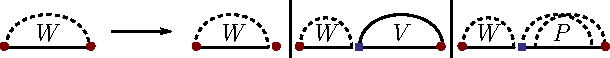
\includegraphics{KnottyPF/recursionW}
\end{equation}
% HJ- this is from our Knotty paper
\textbf{HJ-}In this graphical notation, the RNA sequence is represented as a line with bases as index positions; solid arcs indicate base pairs; and dashed arcs enclose areas containing unconsumed (not decomposed?) structure. 
Red circles represent fixed end points of a region. Blue squares are free indices (i.e. bases that are pivotal for boundary determinations). 
To not clutter the representation, we do not mark end points that can be identified from bases directly before or after them.

Similar changes disambiguate the WB and WP recursions. 
This moves the focus to the decomposition of $P$-fragments. 
\textbf{HJ-} I think we should use $P$-rule instead.
$P$-fragments represent structures $R$ of subsequences $i..l$, where
$i$ and $l$ are paired and part of the same pseudoknot, i.e. in all those structures, there are base pairs $(i,i')$ and $(l',l)$, such that
\begin{enumerate}
\item either $(i,i')$ and $(l',l)$ are crossing each other
\item or $(i,i')$ and $(l',l)$ are both crossing a third base pair $(k,k')$, where $i<k<i'<l'<k'<l$.
\item $(i,i')$ crosses a base pair $(k_1,k_1')$ that crosses $(k_2,k'_2)$ that crosses $(l',l)$ $(i<k_1<k_2<k'_1<k'_2<l)$.
\end{enumerate}
\textbf{HJ-} I believe it would be better to talk about bands instead of single base pairs. \textbf{SW-} My feeling was this is less complex on the level of base pairs. We could mention that this implies the same relation on the level of bands (i.e. there is a band of i.i' and a band of l'.l, ...), or rather we should emphasize that a base pair uniquely determines a band. \textbf{HJ-} I think with current definition of base pairs identifying a band, a simple explanation as you suggested would suffice.

We observe that all these cases are disjoint and form a complete decomposition of CCJ structures, since CCJ structures do not allow three base pairs that all pairwise cross each other and the longest possible chains of crossing base pairs are $4$-chains (third case).

In each case, we decompose the $P$-fragment over [i..l] into two gapped fragments over $[i..j]\cup[k..k']$ and $[j+1..k-1]\cup[k'+1..l]$. 

\textbf{HJ-} I think we can safely replace "gapped fragments" with "gapped regions".

%Gapped fragment: $\RNA{i-j----k-l}{1/10,3/8}$
%
%P-fragment decomposed into two gapped fragments: $\RNA{i-----------l}{1/10,3/8,4/13,7/11}$

For case 1, we achieve crossing of $(i,i')$ and $(l',l)$ if and only if the
base pairs 'span' the gap in their respective fragment. We define, in a gapped
fragment over $[i..j]\cup[k..l]$ ($i\leq j<k\leq l$), a base pair (x,y)
\emph{spans the gap} iff $x\in[i..j]$ and $y\in[k..l]$.

Case 3 applies iff in both gapped fragments, the respective base pairs $(i,i')$ and $(l',l)$ do not span the gap.

In the remaining case 2, one of the base pairs spans the gap and the other does
not. We can arbitrarily break the implied symmetry by requiring $(i,i')$ to
span the gap in its gapped fragment.

\paragraph{Types of gapped fragments}

First of all, note that the decomposition of a P-fragment, can be unambiguous
only, if we strengthen the requirements in the gapped fragments compared to the
PK-fragments of the ambiguous CCJ algorithm.  For the structures represented by
PK-type gapped fragments on $[i..j]\cup[k..l]$ we require that $i$, $j$ and $l$
are paired to respective positions $i'$, $j'$, $l'$. Moreover, each of these
base pairs crosses one of the others.  Note that there are special
cases, where $i=j$ or $k=l$ or both. In these cases, there are only one or two
such base pairs, but the same conditions apply. Moreover, there must be one
base pair that spans the gap. (In comparison, the original CCJ algorithm
required similar conditions only for $i$ and $l$.)

Our considerations give rise to defining four types of gapped
fragments, where
\begin{enumerate}
\item $(i,i')$ spans the gap,
\item $(i,i')$ does not span the gap,
\item $(l',l)$ spans the gap,
\item $(l',l)$ does not span the gap.
\end{enumerate}

Note that this suffices to (de)compose the different types of P-fragments in
the disjoint case distinction that we discussed before.

We observe that the different types of gapped fragments can be distinguished by limiting
the possible decomposition orders in terms of decomposition at the bands L,R,M, and O.
E.g. the constraint (1) is ensured by not decomposing at the left band after the last decomposition at the O-band. 

\textbf{HJ-} It is not clear to me what is meant by ``constraint (1)''.

When we represent the band-decomposition order as word over $\{L,R,M,O\}$, then this corresponds to restricting the prefixes of this word. Therefore, we annotate matrices / fragment types with the allowed prefixes, using a regular expression like notation.

\textbf{HJ-} I am not yet clear with the ``*'' notation. If it is regular-expression-like, then does it mean in $PK_{l*O}$ we can have more than one iteration to get from a $l$ state to an $O$ state?

To ensure the respective properties of the four different PK-type fragments, we could thus denote them by
$PK_{l*O}$, $PK_{o*L}$, $PK_{r*O}$, $PK_{o*R}$; where small letters refer to the negated character class of the corresponding capital letter, e.g. $l$ refers to $[RMO]$.
% 
Note that disambiguation requires to impose even stronger constraints, as we discuss later.
For now, we obtain the following decomposition rule for P-fragments:

\begin{equation}
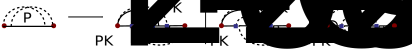
\includegraphics{KnottyPF/recursionP}
\end{equation}

where, generically, fragments $PK.^1$ and $PK.^2$ are decomposed into fragments $PK.$ and $WP$ to account unambiguously for recursive substructure:

\begin{equation}

\includegraphics{KnottyPF/recursionPK12}
\end{equation}

For decomposing fragments like $PK_{l*O}$, in general $PK_{regex}$ it is now crucial to satisfy the band-decomposition-order constraint.
Let us start with the decomposition of $PK_{l*O}$. Generally $PK$-fragements are decomposed into $P_X$-type fragments, where we
need to allow recursive substructure (i.e. $WP$-fragments) between the $P_X$-fragments.

\begin{definition}
The structures represented by a $P_X$-rule over gapped region $[i..j]\cup [k..l]$ satisfy the following properties:
\begin{itemize}
\item all ends $i$, $j$, $k$, and $l$ are paired, but not necessarily to each other.
\item the closing bases at the ``$X$'' side of the gapped region form a base pair%``closed at $X$''
---there is a base pair at the position $X$ ($X\in\{L,R,M,O\}$).
\item there is a base pair that spans the gap $i$ region $j+1..k-1$ -- \textbf{HJ-} I am not clear about the meaning of this part.
\item unless $X=O$, the end bases cannot all be part of the same band (i.e. $i=j$ and $k=l$)n. (Note that we terminate with $O$, unlike the original CCJ recursions, which terminate at $M$.)
\end{itemize}
\end{definition}


We obtain decompositions of PK-fragments like 
\begin{equation}

\includegraphics{KnottyPF/recursionPKlstarO}
\end{equation}
Note that the recursion to $P_O$ already satisfies the constraint due to $l*O$.

We need to further decompose the $P_X$ fragments (which are optionally restricted by regular expressions). Generally, we distinguish three cases by the type of the closing base pair at position $X$. 1) it could close an interior loop in the same band, 2) a multi-loop in the same band (with costs for inner base pairs and unpaired based accounted in WB), or 3) it could `close' the band, i.e. it is the innermost base pair of its band for bands at L,R,O---outermost, in the case of M. Note that the decomposition is disjoint. In the
third case, one changes to decomposing some other band (or terminates the final O-band). Also, in the third case, we allow recursive substructure between bands (WP), which needs to be inserted unambiguously.

Let us quickly handle some details in the unambiguous decomposition of multi-loops within bands (where the recursions operate on gapped fragments):
\begin{equation}
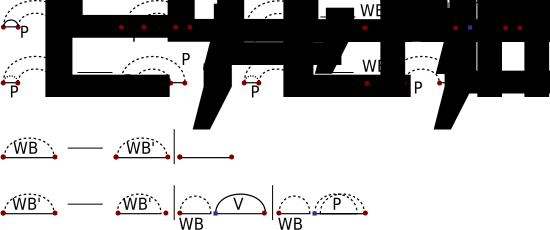
\includegraphics{KnottyPF/recursions-L-mloop}
\end{equation}


It remains to ensure that the order in which bands are decomposed is never ambiguous. Note that in the handling of interior loops and multi-loops within a band, we can simply pass through any constraints on the order of band-decompositions.

\paragraph{Unambiguous decomposition order:}
The original CCJ algorithm already contains restrictions on the band-decomposition order, which are encoded in the rules for decomposition of $P\text{fromX}$-fragments ($X$ in $\{\text{L,R,M,O}\}$). These restrictions are
\begin{itemize}
\item (decomposition at) $R$ cannot be immediately followed by $L$
\item $M$ cannot be immediately followed by $O$
\item $O$ cannot be immediately followed by $M$
\end{itemize} 
The latter two restrictions ensure that the position changes correspond to true changes of the band (in both cases one would just extend the same band). The first restriction is indeed a disambiguation, since immediately successive decompositions at $L$ and $R$ could be exchanged, but it is again required to ensure that position changes introduce band changes, since going back and forth between $L$ and $R$ like $LRL$ would just extend the $L$ band. 

These restrictions in the original CCJ algorithm were necessary for proper scoring, but at the same time ensure unambiguous decomposition. 
%To see this, we go back to the properties of $P_X$-fragments:
%in each structure of a $P_X$-fragment (with the exception of the terminal O-band).


Here are examples for the decomposition of $P_X$:
\begin{equation}
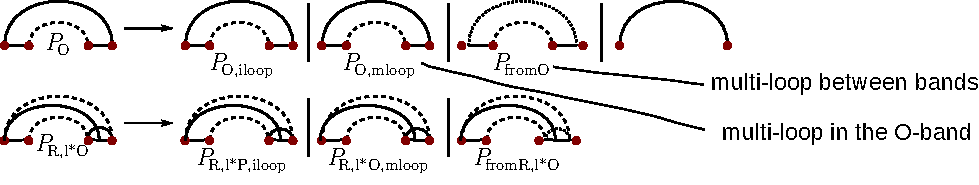
\includegraphics{KnottyPF/recursionPX}
\end{equation}

$P_{fromX}$-fragments are required to change the band; note that we need to unambiguously allow recursive substructure \emph{and} unambiguous band change. For the unconstrained $P_O$, the recursion to the unconstrained $P_\text{fromO}$ works like in the original recursions. 
\begin{equation}
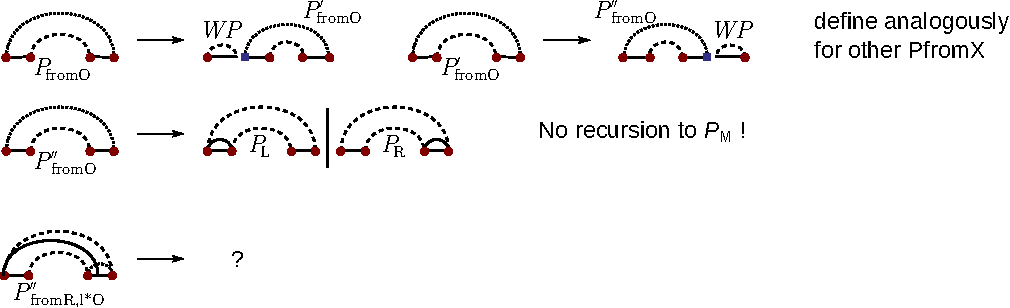
\includegraphics{KnottyPF/recursionPfromX}
\end{equation}

\SW{Replace svg figs with Tikz:}

\begin{equation}
\begin{GRule}
  %LHS
  \GRgapfraglO[right arc/.style={dotted arc}]{$P_{\text{fromR,l*O}}$} 
  \GRdecompTo
  %RHS
  \GRgapfraglO[inner arc/.style={solid arc},ktype/.style=free]{}\GRseclabel{$P_{\text{M,l*O}}$}
  \GRconcatWBefore{k}\GRwfrag[itype/.style=fix]{$W\!P$}\GRrestorelast
  \GRor        
  \GRgapfrag[outer arc/.style={solid arc},ltype/.style=free]{$P_{\text{O}}$} 

  \GRconcat\GRwfrag[ltype/.style=fix]{$W\!P$}
\end{GRule}
\end{equation}


Note that we unambiguously add recursive substructure by adding the substructure (WP-fragments) always between the bands of each transition (note that in each possible transition, but L to R, there is such a unique position between the two bands; for L to R transitions, we do not include substructure).

The set of allowed transitions can be sketched as transition diagram.
Note the asymmetry in the allowed transitions.

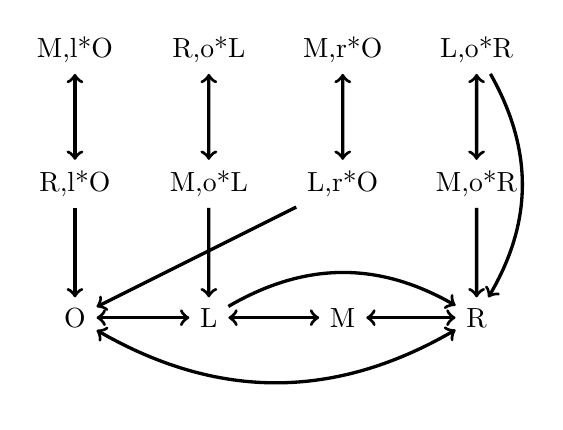
\begin{tikzpicture}[scale=1.7,very thick]
\node (O) at (0,0) {O};
\node (L) at (1,0) {L};
\node (M) at (2,0) {M};
\node (R) at (3,0) {R};
\node (RlO) at (0,1) {R,{l*O}};
\node (MlO) at (0,2) {M,{l*O}};
\node (RoL) at (1,2) {R,{o*L}};
\node (MoL) at (1,1) {M,{o*L}};
\node (LrO) at (2,1) {L,{r*O}};
\node (MrO) at (2,2) {M,{r*O}};
\node (LoR) at (3,2) {L,{o*R}};
\node (MoR) at (3,1) {M,{o*R}};
\draw
  (MlO) edge [<->] (RlO)
  (RlO) edge [->] (O)
  (RoL) edge [<->] (MoL)
  (MoL) edge [->] (L)
%
  (MrO) edge [<->] (LrO)
  (LrO) edge [->] (O)
  (LoR) edge [<->] (MoR)
  (LoR) edge [->,bend left] (R)
  (MoR) edge [->] (R)
%
  (R) edge [<->,bend left] (O)
  (R) edge [<->] (M)
  (L) edge [->,bend left] (R)
  (L) edge [<->] (M)
  (L) edge [<->] (O);
\end{tikzpicture}

\SW{
\textbf{Not elaborated yet:} How to handle the $PK_{o*L}$, $PK_{r*O}$, and $PK_{o*R}$ fragments?
}

\SW{Idea: We should formally define \emph{band decomposition order (bdo)} (as a word over $\{L,R,M,O\}$ for decompositions of a structure
represented by $P$. Proving the uniqueness of bdo (given our restrictions) would be an essential step to showing the uniqueness of the recursions. For showing completenes, it is important to precisely define all the fragments (in terms of the represented structures).}

\end{document}
